\documentclass[tikz]{standalone}

\colorlet{FilledSurface}{blue!20}
\colorlet{FilledSurfaceGroupOne}{blue!20}
\colorlet{FilledSurfaceGroupTwo}{red!20}
\colorlet{FilledSurfaceGroupThree}{green!20}
\colorlet{FilledSurfaceGroupFour}{magenta!20}
\colorlet{FormulaBackground}{green!10}
\colorlet{FormulaFrame}{green}


\usetikzlibrary{calc, angles, intersections}

\begin{document}
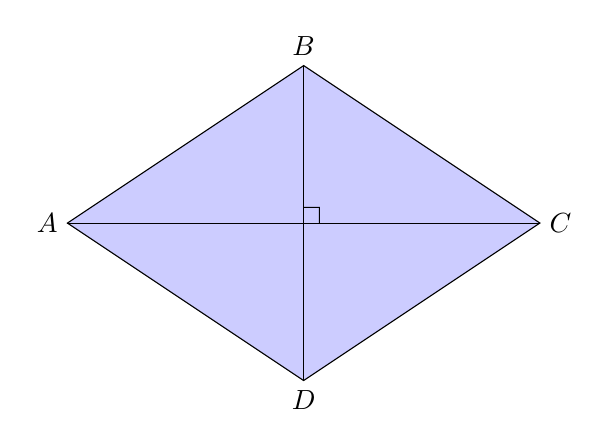
\begin{tikzpicture}

\coordinate (A) at (0, 0);
\coordinate (B) at (3, 2);
\coordinate (C) at (6, 0);
\coordinate (D) at (3, -2);
\draw[fill=FilledSurfaceGroupOne]
    (A) node[left]{$A$}
    -- (B) node[above]{$B$}
    -- (C) node[right]{$C$}
    -- (D) node[below]{$D$}
    -- cycle;

\coordinate (H) at (B |- A);

\draw[name path=BD] (B) -- (D);
\draw[name path=AC] (A) -- (C);
\path [name intersections={of=AC and BD, by=I}];
\path pic [draw,angle radius=2mm] {right angle = B--I--C};

\end{tikzpicture}
\end{document}


